\section{Technische Konzepte}\label{technische_konzepte}
Im kommenden Kapitel wird zunächst ein mögliches Konzept für die\textit{ Klassifizierung von Software} vorgestellt, welche in der Eingangslogistik stattfindet. In Kapitel \ref{umgebungssuche} wird ein Such-Algorithmus skizziert, welcher die \textit{automatische Erkennung von Softwarebedarf} unterstützt. Im letzten Kapitel werden drei Kommunikationskonzepte vorgestellt, welche den Ablauf der Kommunikation zwischen dem Fahrzeug, dem Server und Service Providern im Kontext automatischen Parkens skizzieren und im Prototypen verwendet werden.
\subsection{Klassifizierung von Software}\label{sw_klassifizierung}
Das Ziel der Software Klassifikation ist es, den Fahrzeughaltern beim Kauf unterstützende Kennzahlen zur Verfügung zu stellen, anhand welcher sie sinnvollere Kaufentscheidungen treffen können und somit potentiell einen größeren Wert von der gekauften Software erhalten.

\subsubsection{Berechtigungen}
Eine dieser Kennzahlen ist die Anzahl genutzter Berechtigungen des Fahrzeugs. Nicht nur die Anzahl, sondern auch der Umfang einzelner Berechtigungen können Kunden vom Kauf abschrecken.\cite[Vgl. S. 107]{android} Eine Berechtigung erteilt einer Software die Erlaubnis, auf einzelne Systeme bzw. APIs des Fahrzeugs zugreifen zu dürfen und steigern hierdurch die Sicherheit dessen. Sie werden von Entwicklern zu einer Software hinzugefügt und müssen beim Kauf die Zustimmung des Fahrzeughalters erhalten, damit diese im vollen Umfang vom Fahrzeug genutzt werden kann. Stimmen Fahrzeughalter Berechtigungen nicht zu, kann die entsprechende Software nicht gekauft werden. Durch die Verwendung von Berechtigungen kann die Sicherheit von Softwares gesteigert werden da sie verhindern, dass eine Software ohne weiteres auf alle Daten und Systeme des Fahrzeugs zugreifen kann. Im Kontext autonomer Fahrzeuge können mögliche Berechtigungen von der Architektur dieser abgeleitet werden, welche in Abbildung \hyperref[img:av_architecture]{9} dargestellt wird. 
\begin{figure}[H]
	\centering
	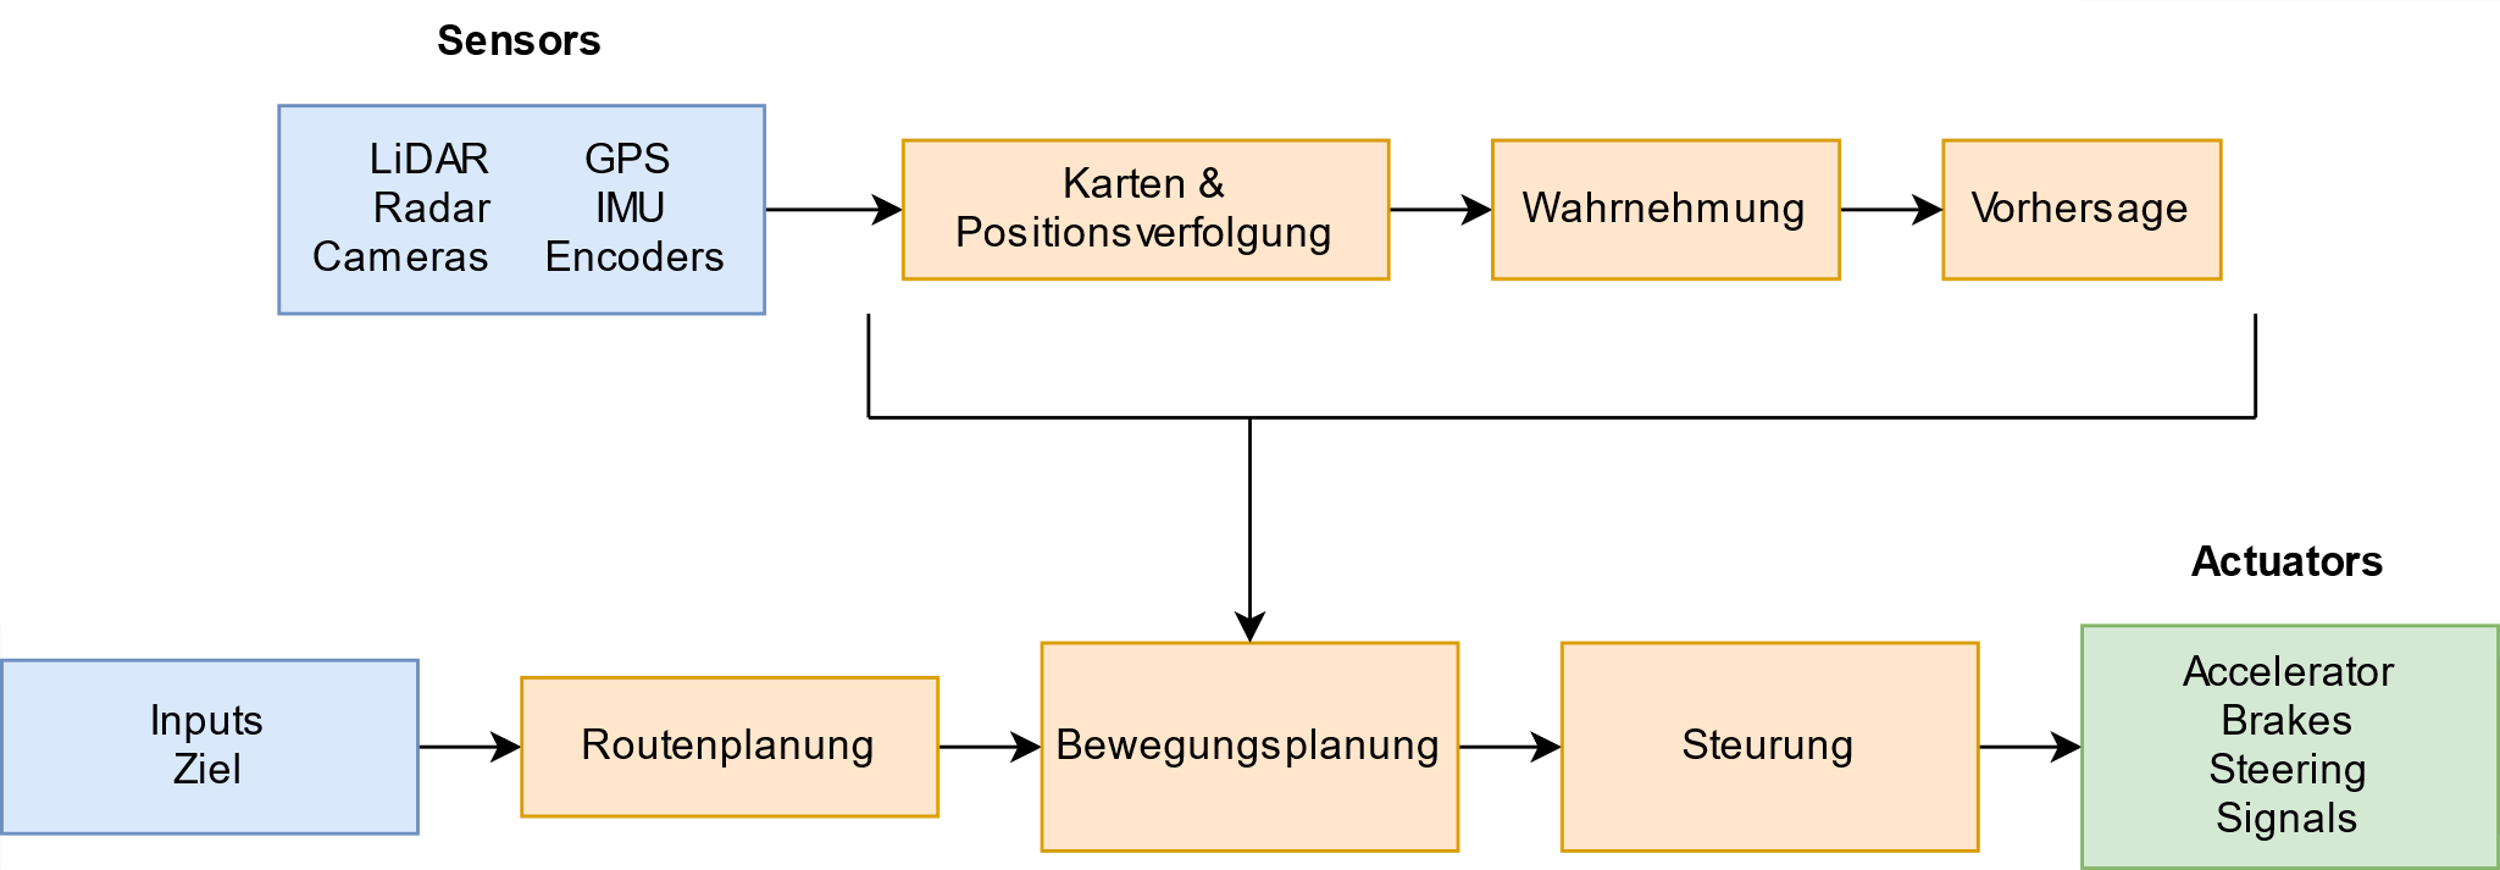
\includegraphics[width=0.95\columnwidth]{pictures/arichtecture_AV.png}
	\label{img:av_architecture}
	\caption{Jeff Schneider: Architecture of Autonomous Vehicles}
\end{figure}

Damit Berechtigungen die Fahrzeughalter davor schützen persönliche Informationen unfreiwillig zu teilen und einer Software so zu viel "Macht" über das Fahrzeug zu geben, sollte der Umfang von Berechtigungen möglichst klein gehalten werden. So sollte jede Sensorgruppe des Fahrzeugs eigene Berechtigungen haben, da die Art der aufgenommenen Informationen sich voneinander unterscheidet. Durch das Auslesen des GPS-Sensors kann die Position des Fahrzeugs kontinuierlich aufgezeichnet werden, während dies über den Radar nicht möglich ist. Würde alle Sensoren über die gleiche Berechtigung zugänglich sein, würde dies dementsprechend eine Sicherheitslücke darstellen.\\

Neben der Privatsphäre der Fahrzeughalter ist vor allem die Sicherheit von Fahrzeuginsassen wichtig. Wird eine Software entwickelt, welche die Wahrnehmung, Vorhersage, Zieleingabe, Routenplanung, Bewegungsplanung, die Steuerung oder einzelne Aktuatoren beeinflusst, kann dies die Sicherheit der Insassen gefährden. Softwares, die diese Systeme nur auslesen aber nicht direkt beeinflussen haben keine Auswirkung auf die Fahrsicherheit. Daher sollte jedes System jeweils zwei einzelne Berechtigungen haben. Durch die eine kann ein System ausgelesen werden. Durch die andere können Systeme beeinflusst werden, wodurch aktiv in die Fahraufgabe eingegriffen wird.\\

Neben Berechtigungen, die einzelne Systeme eines Fahrzeugs benötigen, sollten auch weitere Services des Fahrzeugs nur durch die Nutzung von Berechtigungen möglich sein. Eine Berechtigung für die Nutzung des Internets ist sinnvoll, da Softwares hierdurch nicht wahllos Nutzerdaten speichern können. Auch die Kommunikation mit anderen Akteuren des Straßenverkehrs sollte über eine Berechtigung beschränkt werden, um den Fahrer vor 'Spam' zu schützen.

\subsubsection{Softwarekennzahlen}
Neben der Art und Anzahl genutzter Berechtigungen einer Software, können auch andere Kennzahlen einer Software den Fahrzeughalter bei der Kaufentscheidung unterstützen. Einige dieser Kennzahlen können von den im Businessmodel beschriebenen Nutzenversprechen abgleitet werden \textit{(Kapitel \ref{nv})}.\\

Um darzustellen, dass die Lebenszeit das Autos verlängert wird \textit{(NV-4)} kann ein Wert berechnet werden, der aussagt wie gut eine Software die einzelnen Autoteile \textit{(Motor, Gertiebe, Reifen etc.)} schont. Die Berechnung dieses Werts kann in Simulationsumgebungen wie Carla erfolgen. Zunächst müssen zwei Fahrzeuge simuliert werden, von denen das eine die zu prüfende Software installiert hat und das andere nicht. Beide Fahrzeuge sollen die der Software hinzugefügten Szenarien, welche der Software beigefügt wurden, durchfahren und dabei bestimmte Werte wie die Reifenreibung, die Dämpfungsrate oder andere messen. Durch einen Vergleich der gemessenen Werte kann prozentual angegeben werden, wie stark eine Software bestimmte Teile des Fahrzeugs schont \textbf{oder auch eben nicht}. Um Fahrzeughaltern vor Augen zu führen wie viel Zeit durch eine Software gewonnen werden kann \textit{(NV-6)}, sollte ein Zeitwert berechnet werden, welcher die durchschnittlich autonom zurückgelegte Zeit einer Software bestimmt. Die Berechnung sollte auf Basis realer Nutzungsdaten durchgeführt werden. Neben der durchschnittlichen selbstständigen Fahrzeit einer Software kann auch die Anzahl an Interaktionen mit der Autoumwelt ein ausschlaggebender Faktor für den Kauf einer Software sein. Weiter Kennzahlen können sein:
\begin{itemize}
	\item[\textbf{1.}]\textbf{Anzahl an Downloads und Deinstallationen}
	\item[\textbf{2.}]\textbf{Benötigter Speicherplatz der Softwrae}
	\item[\textbf{3.}]\textbf{Bewertung der Software durch Fahrzeughalter}
\end{itemize}

Es ist sinnvoll die Bestimmung einzelner Kennzahlen Regionsabhängig zu gestalten, da diese sonst irreführend sein können: Nehmen wir an, eine Software soll das Fahren in der Innenstadt ermöglichen. Wohnt der Fahrzeughalter nicht im Umkreis einer Stadt, würde ihm die Software nichts sonderlich viel bringen. Durch die hohe Anzahl gesparter Stunden ist der Fahrzeughalter überzeugt und kauft sich diese dennoch. Um derartige Fälle zu verhindern, sollt die Berechnungen von Kennzahlen an die jeweilige Region des Fahrzeugs angepasst sein. \\\\
Die vorgestellten Berechtigungen und Softwarekennzahlen sollen im Shop zu jeder Software angezeigt werden, damit Fahrzeughalter sich einen Eindruck einer Software aufbauen können der sie bei der Kaufentscheidung unterstützt. Außerdem können Kennzahlen und Berechtigungen auch als Such-Filter im Shop verwendet werden, was die Suche nach bestimmten Softwares im Shop erleichtern kann. 

\subsection{Umgebungsbedingte Softwaresuche}\label{umgebungssuche}
In Kapitel \ref{wsk} wurden mehrere Möglichkeiten aufgezählt, mit denen der Softwarebedarf eines Fahrzeugs automatisch bestimmt werden kann. Die im folgenden vorgestellte Umgebungssuche soll einem Fahrzeughalter Softwares vorschlagen, welche in der Umgebung des Fahrzeugs des öfteren von anderen Verkehrsteilnehmern gekauft oder genutzt werden.\\\\
Die Umgebungssuche beginnt mit dem Verschicken einer Nachricht vom Fahrzeug an den Server. In dieser Nachricht ist das Manifest des Fahrzeugs enthalten, auf welchem unter anderem eine Liste aller installierter Softwares des Fahrzeugs zu finden ist. Außerdem werden Fahrdaten verschickt durch welche ersichtlich wird, in welchen Regionen sich das Fahrzeug zuletzt aufgehalten hat. Der Server sucht innerhalb dieser Regionen nach Softwares, die dort von anderen Fahrzeughaltern gekauft wurden und noch nicht auf dem anfragenden Fahrzeug installiert sind. Ist die Suche abgeschlossen wird geprüft, ob die gefundenen Softwares einen Mehrwert für das Fahrzeug bieten. Um dies zu bestimmen, können die einer Software beigelegten Open Scenario Dateien genutzt werden und in einer Simulation durchfahren werden.\\

Zunächst wird eine virtuelle Instanz des Fahrzeugs anhand des versendeten Manifests erstellt \textit{(Originalinstanz)}. Für jede gefundene Software wird eine weitere Instanz des Fahrzeugs erstellt, auf welcher die jeweilige Software zusätzlich installiert wird\textit{(Neue Instanzen)}. Nach dem erstellen der virtuellen Fahrzeuge, durchlaufen die Originalinstanz und die neue Instanzen die jeweiligen Szenarien der Softwares. Durch einen Vergleich der Simulationen soll festgestellt werden, ob eine Software positive, negative oder überhaupt keine Auswirkungen auf das Fahrverhalten des Fahrzeugs in den Szenarien hat. Positiv ist, wenn das Fahrzeug die Situation nun selbstständig durchfahren kann oder dies Ressourcenschonender tut. Negativ  ist es, wenn die Situation durch die neue Software nicht weiter durchfahren wird oder die neue Software zum durchfahren der Situation nicht vom Fahrzeug ausgewählt wird. Dies kann bedeuten, dass auf dem Fahrzeug bereits eine Software installiert ist, welche die Situation bereits abdeckt.

\subsection{Kommunikationsprotokolle}\label{4.2}
Damit Software heruntergeladen und anschließend genutzt werden kann, müssen das Fahrzeug, der Software Shop und auch potentiell weitere Akteure des Straßenverkehr \textit{(Autos, Ampeln, Service Provider, oA.)} miteinander kommunizieren. Damit diese Kommunikation sicher und geordnet ist, werden drei Kommunikationsprotokolle erstellt die im Prototypen implementiert werden können. Die in den Protokollen gelb gefüllten Ovale repräsentieren einzelne Module des Prototypen, welche in Kapitel \ref{prototyp} vorgestellt werden.

\subsubsection{Kommunikationsprotokoll: Selbstständiger Softwarekauf}
\begin{wrapfigure}{R}{0.5\textwidth}
	\centering
	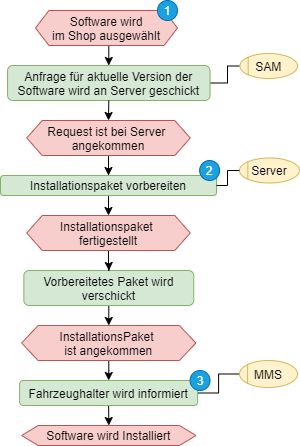
\includegraphics[width=0.48\textwidth]{pictures/konzept-Eigene-Installation.png}	\label{img:eigenstaendigIns}
	\caption{Eigenständige Installation von Software}
\end{wrapfigure}
Das in Abbildung \hyperref[img:eigenstaendigIns]{10} dargestellte Protokoll stellt den Kommunikationsablauf beim Kauf einer spezifischen Software dar. Der Fahrzeughalter kann im Shop nach Softwares suchen, indem der Name einer Software gesucht wird oder Suchfilter verwendet werden. Wurde eine Software ausgewählt \textit{(1)}, wird eine Installationsanfrage für diese an den Server geschickt. Kann die Software auf dem Fahrzeug installiert werden, bereitet der Server ein \textbf{Installationspaket} vor \textit{(2)}. In diesem ist die Software, eine neue Version des Manifests und das Angebot für die Software enthalten. Ist das Installationspaket vorbereitet, wird es an das Fahrzeug verschickt und der Fahrzeughalter wird über die Mensch Maschine Schnittstelle über darüber informiert\textit{(3)}. Abschließend wird die Software auf dem Fahrzeug installiert und der Fahrzeughalter kann sie nutzen.
\clearpage
\subsubsection{Kommunikationsprotokoll: Installationsvorschlag vom Service Provider}
In Abbildung \hyperref[img:installationsProtokollExtern]{11} wird dargestellt, wie ein Service Provider einem Fahrzeug eine Software vorschlagen kann. Die Notwendigkeit hierfür besteht, da zur Nutzen eines Services jeweils eine bestimmte Software notwendig ist. Vorzustellen sei folgende Situation: Ein Fahrzeughalter möchte in der Oldenburger Innenstadt einkaufen gehen und muss hierfür sein Fahrzeug parken. Über das Navigationssystem wählt er einen Parkplatz aus den das Fahrzeug daraufhin ansteuert. Um ein Parkticket für diesen Parkplatz kaufen und das Fahrzeug automatisch einparken zu können, benötigt dieses eine bestimmte Software. Am Parkplatz angekommen, fährt das Fahrzeug in das Sichtfeld des Parkautomaten, auch \textit{Registrierungszone} genannt \textit{(1)}. Wird ein Fahrzeug erkannt, registriert sich der Parkautomat beim Fahrzeug. Ist die Registrierung im Fahrzeug angekommen überprüft der Software Applikation Manager, ob die für den Service benötigte Software bereits auf dem Fahrzeug installiert\textit{(2)}.\\
Ist dies der Fall, wird zusätzlich überprüft ob die installierte Version der Software aktuell ist. Wenn ja, kann der Service genutzt werden - wie die Nutzung eines Service abläuft, wird im dritten und letzten Kommunikationsprotokoll dargestellt. Ist die Software noch nicht Installiert oder die installierte Version ist nicht mehr aktuell wird der Fahrzeughalter gefragt, ob er die Software Aktualisieren bzw. Kaufen möchte \textit{(4)}. Er kann das ihm vorgestellte Angebot entsprechend seiner Bedürfnisse für die Software anpassen \textit{(Leihe statt Kauf, etc.)} und seine Entscheidung durch eine Eingabe in der Mensch Maschine Schnittstelle bestätigen. Wird die Anfrage abgelehnt, wird keine Software installiert. Das Fahrzeug verlässt die Registrierungszone wieder und kann nicht auf dem Parkplatz parken. Nimmt der Fahrzeughalter die Anfrage hingegen an, sendet das Fahrzeug eine Installationsanfrage an den Server.  Der Server nimmt die Anfrage an und erstellt ein Installationspaket für die entsprechende Software \textit{(5)}. Das erstellte Paket wird an das Fahrzeug gesendet, auf diesem installiert und das Fahrzeug kann den angebotenen Park-Service nutzen. 
\begin{figure}[!h]
	\centering
	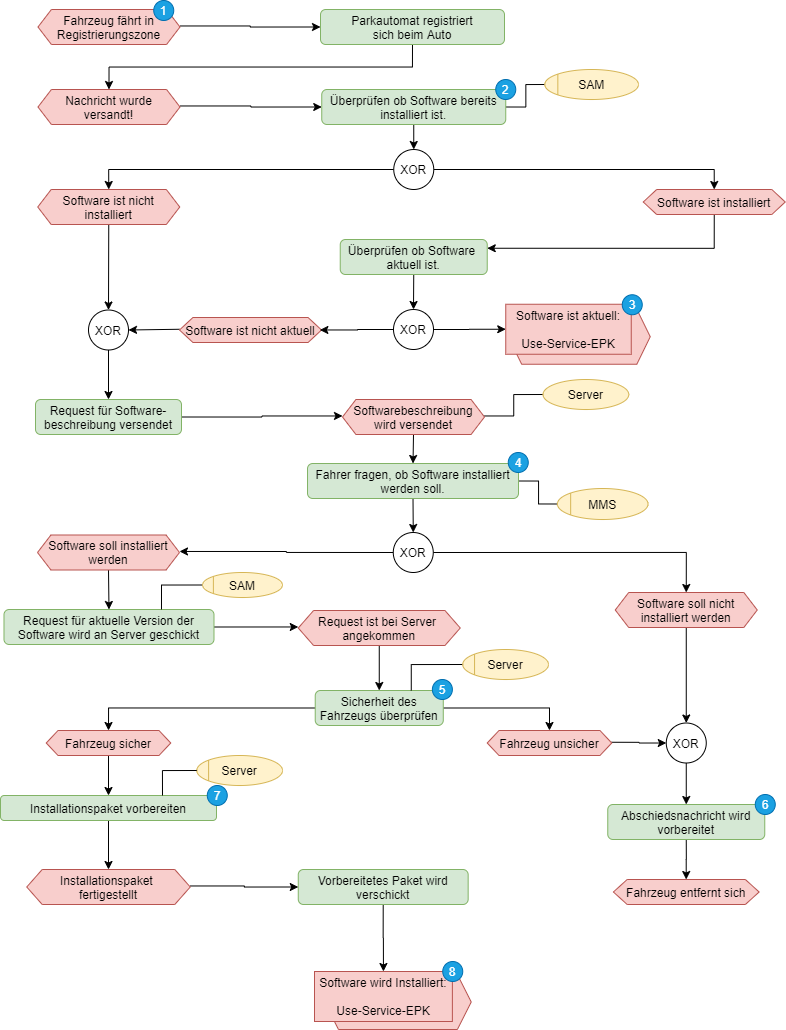
\includegraphics[width=\columnwidth]{pictures/konzept-Installationsprozess.png}
	\label{img:installationsProtokollExtern}
	\caption{Installationsprozess von Software}
\end{figure}
\subsubsection{Kommunikationsprotokoll: Nutzung eines Service}
Abbildung \hyperref[img:nutzung]{12} zeigt den Kommunikationsablauf zwischen einem Fahrzeug und einem Service Provider Actor \textit{(bspw. ein Parkautomat)}. Der dargestellte Ablauf findet statt, wenn ein Fahrzeug einen Service nutzen möchte und die aktuelle Version der hierfür notwendigen Software bereits auf dem Fahrzeug installiert ist \textit{(1)}. Der Service wird über die Mensch Maschine Schnittstelle zur Nutzung vorgeschlagen \textit{(2)} und der Fahrer kann entscheiden, ob er dies tun möchte oder nicht. Die Entscheidung des Fahrers wird an den Parkautomaten gesendet \textit{(3)}, welcher die Entscheidung evaluiert und dementsprechend dem Fahrzeug entweder einen Parkplatz zuweist oder es verabschiedet. Die jeweilige Antwort wird an das Fahrzeug gesendet und über die MMS angezeigt. Das Fahrzeug plant die kommende Bewegung und fährt dementsprechend entweder zu dem ihm zugewiesenen Parkplatz oder verlässt die Registrierungszone wieder.
\begin{figure}[!h]
	\centering
	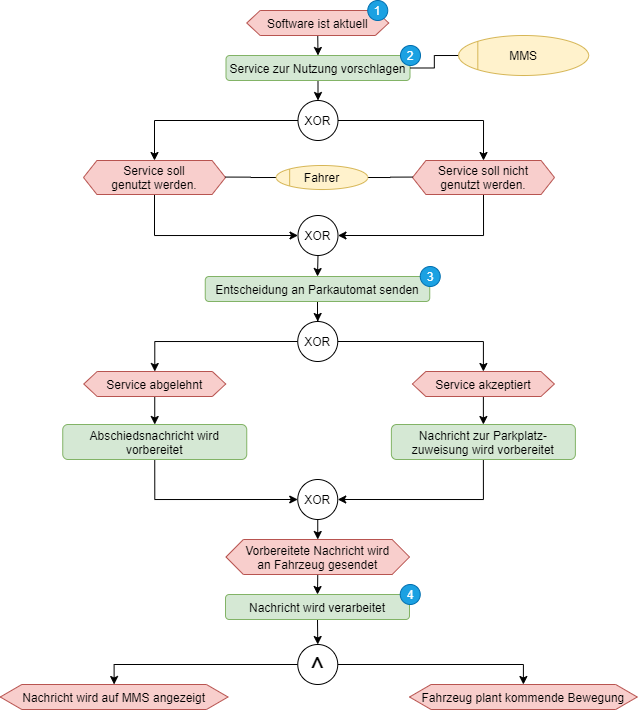
\includegraphics[width=0.8\columnwidth]{pictures/konzept-Nutzungsprozess.png}
	\caption{Nutzungsprozess von Software}
	\label{img:nutzung}
\end{figure}
\clearpage
\subsection{Ausblick}
Die in diesem Kapitel erstellten Konzepte wurden mit der Intention entwickelt, einzelne Bausteine der Wertschöpfungskette zu detaillieren und im Prototypen implementiert zu werden. Die Identifikation von Berechtigungen für einzelne Systeme eines Fahrzeugs bieten eine geeignete Grundlage, die Sicherheit intelligenter Fahrzeuge zu unterstützen. Fahrzeughalter können durch diese und weitere Kennzahlen bessere Kaufentscheidungen treffen und ihr Fahrzeug so erweitern, dass es auf deren Ansprüche angepasst ist. Die Kommunikationsprotokolle wurden erstellt, um einen Ablauf für den Prototypen aufstellen und nachverfolgen zu können. Die Kommunikationsprotokolle, die im Forschungsseminar erarbeitete Softwarearchitektur und auch weitere in der Arbeit gewonnene Erkenntnisse und Ideen werden im Prototypen eingebunden und visuell veranschaulicht.\\\\\\\\\\\\\\\\\\\\\\